
\documentclass[template=tabling,81pt,headonall]{azmoon}
\usepackage{xepersian}
\usepackage{amsfonts}
\usepackage{graphicx}
\graphicspath{ {./images/} }
\settextfont{Yas}
\setdigitfont{A Iranian Sans}
\usepackage{fontawesome5}

\printanswers
    \teacher{محمد صالح علی اکبری}
    \teachertitle{دبیر}
    \city{گناباد}
    \schooltitle{متوسطه دوره دوم}
    \school{شاهد امام (ره)}
    \grade{دهم}
    \branch{۱۵۱}
    \topic{ریاضی}
    \examdate{آذر ۱۴۰۲}
    \answertime{80 دقیقه}
    \begin{document}
	\begin{questions}
		\nointerlineskip%
		\vskip-\baselineskip
		\question{%
متن، زیر متن و فرا متن تبلیغ زیر را تشریخ کنید. \\
\includegraphics[scale = 0.31]{images}}\question{%
تصاویر زیر مربوط به دو تبلیغ از بستنی شرکت میهن است. با توجه به این که این تبلیغ برای داخل کشور طراحی شده متن، زیر متن و فرامتن آن را تحلیل کنید. \\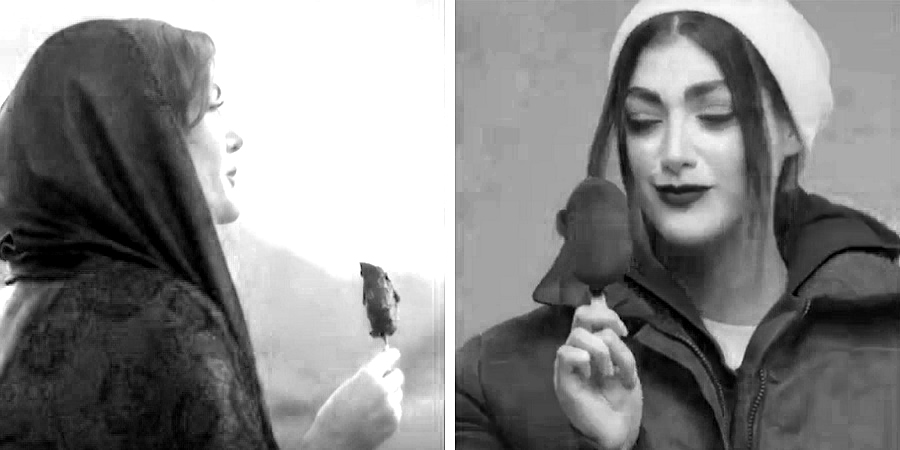
\includegraphics[scale = 0.15]{Unt5747jytkiyksgitled}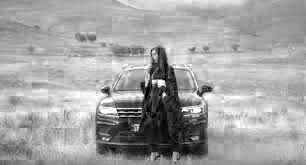
\includegraphics[scale = 0.3]{بستنی}‌
\\‌
\\}\question{%
متن زیر متن و فرامتن تبلیغ زیر را بیان کنید. برداشت شما از کشوری که این تبلیغ در آن استفاده شده است چیست؟ \\
\includegraphics[scale = 0.31]{Screenshot 2023-12-20 010718}‌
\\‌
\\}\question{%
با توجه به این که واکنش‌ها به تبلیغ شرکت میهن قابل پیش بینی بوده است هدف اصلی این شرکت برای هزینه برای این تبلیغ چه بوده است؟ نظر خود را بنویسید.‌
\\‌
\\‌
\\‌
\\‌
\\}\end{questions}
    \end{document}
    